\section{zesto-llc.cpp File Reference}
\label{zesto-llc_8cpp}\index{zesto-llc.cpp@{zesto-llc.cpp}}
{\tt \#include $<$limits.h$>$}\par
{\tt \#include \char`\"{}thread.h\char`\"{}}\par
{\tt \#include \char`\"{}stats.h\char`\"{}}\par
{\tt \#include \char`\"{}zesto-core.h\char`\"{}}\par
{\tt \#include \char`\"{}zesto-opts.h\char`\"{}}\par
{\tt \#include \char`\"{}zesto-cache.h\char`\"{}}\par
{\tt \#include \char`\"{}zesto-prefetch.h\char`\"{}}\par
{\tt \#include \char`\"{}zesto-uncore.h\char`\"{}}\par
{\tt \#include \char`\"{}zesto-exec.h\char`\"{}}\par
{\tt \#include \char`\"{}zesto-commit.h\char`\"{}}\par


Include dependency graph for zesto-llc.cpp:\nopagebreak
\begin{figure}[H]
\begin{center}
\leavevmode
\includegraphics[width=420pt]{zesto-llc_8cpp__incl}
\end{center}
\end{figure}
\subsection*{Functions}
\begin{CompactItemize}
\item 
struct {\bf cache\_\-t} $\ast$ {\bf cache\_\-create\_\-llc} (struct {\bf core\_\-t} $\ast$const core, const char $\ast$const name, const bool read\_\-only, const int sets, const int assoc, const int linesize, const char rp, const char ap, const char wp, const char wc, const int banks, const int bank\_\-width, const int latency, const int WBB\_\-size, const int MSHR\_\-size, const int MSHR\_\-banks, const int begin\_\-index, const int end\_\-index, struct {\bf cache\_\-t} $\ast$const next\_\-level\_\-cache, struct {\bf bus\_\-t} $\ast$const next\_\-bus)
\item 
void {\bf LLC\_\-reg\_\-stats} (struct {\bf stat\_\-sdb\_\-t} $\ast$const sdb, struct {\bf cache\_\-t} $\ast$const cp)
\item 
static int {\bf prefetch\_\-filter\_\-lookup} (struct {\bf prefetch\_\-filter\_\-t} $\ast$const p, const {\bf md\_\-paddr\_\-t} addr)
\item 
static void {\bf prefetch\_\-filter\_\-update} (struct {\bf prefetch\_\-filter\_\-t} $\ast$const p, const {\bf md\_\-paddr\_\-t} addr, const int useful)
\item 
struct {\bf cache\_\-line\_\-t} $\ast$ {\bf cache\_\-is\_\-hit\_\-llc} (struct {\bf cache\_\-t} $\ast$const cp, const enum {\bf cache\_\-command} cmd, const {\bf md\_\-paddr\_\-t} addr, struct {\bf core\_\-t} $\ast$const core)
\item 
static struct {\bf cache\_\-line\_\-t} $\ast$ {\bf cache\_\-peek\_\-llc} (const struct {\bf cache\_\-t} $\ast$const cp, const {\bf md\_\-paddr\_\-t} addr)
\item 
void {\bf cache\_\-insert\_\-block\_\-llc} (struct {\bf cache\_\-t} $\ast$const cp, const enum {\bf cache\_\-command} cmd, const {\bf md\_\-paddr\_\-t} addr, {\bf core\_\-t} $\ast$const core)
\item 
struct {\bf cache\_\-line\_\-t} $\ast$ {\bf cache\_\-get\_\-evictee\_\-llc} (struct {\bf cache\_\-t} $\ast$const cp, const {\bf md\_\-paddr\_\-t} addr, {\bf core\_\-t} $\ast$const core)
\item 
static void {\bf cache\_\-heap\_\-balance} (struct {\bf cache\_\-action\_\-t} $\ast$const pipe, const int insert\_\-position)
\item 
static void {\bf cache\_\-heap\_\-remove} (struct {\bf cache\_\-action\_\-t} $\ast$const pipe, const int pipe\_\-num)
\item 
int {\bf cache\_\-enqueuable\_\-llc} (const struct {\bf cache\_\-t} $\ast$const cp, const int thread\_\-id, const {\bf md\_\-paddr\_\-t} addr)
\item 
void {\bf cache\_\-enqueue\_\-llc} (struct {\bf core\_\-t} $\ast$const core, struct {\bf cache\_\-t} $\ast$const cp, struct {\bf cache\_\-t} $\ast$const prev\_\-cp, const enum {\bf cache\_\-command} cmd, const int thread\_\-id, const {\bf md\_\-addr\_\-t} PC, const {\bf md\_\-paddr\_\-t} addr, const {\bf seq\_\-t} action\_\-id, const int MSHR\_\-bank, const int MSHR\_\-index, void $\ast$const op, void($\ast$const cb)(void $\ast$), void($\ast$const miss\_\-cb)(void $\ast$, int), bool($\ast$const translated\_\-cb)(void $\ast$, {\bf seq\_\-t}), {\bf seq\_\-t}($\ast$const get\_\-action\_\-id)(void $\ast$))
\item 
static int {\bf WBB\_\-available} (const struct {\bf cache\_\-t} $\ast$const cp, const {\bf md\_\-paddr\_\-t} paddr)
\item 
static void {\bf WBB\_\-insert} (struct {\bf cache\_\-t} $\ast$const cp, struct {\bf cache\_\-line\_\-t} $\ast$const cache\_\-block)
\item 
static void {\bf WBB\_\-victim\_\-insert} (struct {\bf cache\_\-t} $\ast$const cp, struct {\bf cache\_\-line\_\-t} $\ast$const cache\_\-block)
\item 
static int {\bf MSHR\_\-available} (const struct {\bf cache\_\-t} $\ast$const cp, const {\bf md\_\-paddr\_\-t} paddr)
\item 
static struct {\bf cache\_\-action\_\-t} $\ast$ {\bf MSHR\_\-allocate} (struct {\bf cache\_\-t} $\ast$const cp, const {\bf md\_\-paddr\_\-t} paddr, const enum {\bf cache\_\-command} cmd)
\item 
static void {\bf dummy\_\-callback} (void $\ast$p)
\item 
void {\bf fill\_\-arrived\_\-llc} (struct {\bf cache\_\-t} $\ast$const cp, unsigned long long int address)
\item 
static void {\bf fill\_\-heap\_\-balance} (struct {\bf cache\_\-fill\_\-t} $\ast$const pipe, const int insert\_\-position)
\item 
static void {\bf fill\_\-heap\_\-remove} (struct {\bf cache\_\-fill\_\-t} $\ast$const pipe, const int pipe\_\-num)
\item 
static bool {\bf cache\_\-fillable\_\-llc} (const struct {\bf cache\_\-t} $\ast$const cp, const {\bf md\_\-paddr\_\-t} paddr)
\item 
static void {\bf cache\_\-fill\_\-llc} (struct {\bf cache\_\-t} $\ast$const cp, const enum {\bf cache\_\-command} cmd, const {\bf md\_\-paddr\_\-t} paddr, struct {\bf core\_\-t} $\ast$core)
\item 
void {\bf cache\_\-process\_\-llc} (struct {\bf cache\_\-t} $\ast$const cp)
\item 
static void {\bf cache\_\-prefetch\_\-llc} (struct {\bf cache\_\-t} $\ast$const cp)
\item 
static void {\bf prefetch\_\-controller\_\-update\_\-llc} (struct {\bf cache\_\-t} $\ast$const cp)
\item 
void {\bf step\_\-LLC\_\-PF\_\-controller} (struct {\bf uncore\_\-t} $\ast$const uncore)
\item 
void {\bf prefetch\_\-LLC} (struct {\bf uncore\_\-t} $\ast$const uncore)
\item 
void {\bf uncore\_\-utilize} (struct {\bf cache\_\-t} $\ast$const cp)
\end{CompactItemize}


\subsection{Function Documentation}
\index{zesto-llc.cpp@{zesto-llc.cpp}!cache\_\-create\_\-llc@{cache\_\-create\_\-llc}}
\index{cache\_\-create\_\-llc@{cache\_\-create\_\-llc}!zesto-llc.cpp@{zesto-llc.cpp}}
\subsubsection[{cache\_\-create\_\-llc}]{\setlength{\rightskip}{0pt plus 5cm}struct {\bf cache\_\-t}$\ast$ cache\_\-create\_\-llc (struct {\bf core\_\-t} $\ast$const  {\em core}, \/  const char $\ast$const  {\em name}, \/  const bool {\em read\_\-only}, \/  const int {\em sets}, \/  const int {\em assoc}, \/  const int {\em linesize}, \/  const char {\em rp}, \/  const char {\em ap}, \/  const char {\em wp}, \/  const char {\em wc}, \/  const int {\em banks}, \/  const int {\em bank\_\-width}, \/  const int {\em latency}, \/  const int {\em WBB\_\-size}, \/  const int {\em MSHR\_\-size}, \/  const int {\em MSHR\_\-banks}, \/  const int {\em begin\_\-index}, \/  const int {\em end\_\-index}, \/  struct {\bf cache\_\-t} $\ast$const  {\em next\_\-level\_\-cache}, \/  struct {\bf bus\_\-t} $\ast$const  {\em next\_\-bus})\hspace{0.3cm}{\tt  [read]}}\label{zesto-llc_8cpp_727c4cbf039edb120fe825803e69067f}




Definition at line 90 of file zesto-llc.cpp.

References cache\_\-t::addr\_\-shift, cache\_\-t::allocate\_\-policy, cache\_\-t::assoc, cache\_\-t::bank\_\-mask, cache\_\-t::bank\_\-shift, cache\_\-t::bank\_\-width, cache\_\-t::banks, cache\_\-t::blocks, cache\_\-t::check\_\-for\_\-MSHR\_\-fill\_\-work, cache\_\-t::check\_\-for\_\-work, cache\_\-t::core, cache\_\-t::core\_\-lookups, cache\_\-t::core\_\-misses, fatal(), cache\_\-t::fill\_\-num, cache\_\-t::fill\_\-pipe, cache\_\-t::heap\_\-size, cache\_\-t::latency, cache\_\-t::linesize, cache\_\-t::log2\_\-assoc, cache\_\-t::MSHR, cache\_\-t::MSHR\_\-banks, cache\_\-t::MSHR\_\-mask, cache\_\-t::MSHR\_\-size, mytoupper(), cache\_\-t::name, cache\_\-line\_\-t::next, cache\_\-t::next\_\-bus, cache\_\-t::next\_\-level, NO\_\-WRITE\_\-ALLOC, num\_\-threads, cache\_\-t::pipe, cache\_\-t::pipe\_\-num, cache\_\-t::read\_\-only, REPLACE\_\-CLOCK, REPLACE\_\-LRU, REPLACE\_\-MRU, REPLACE\_\-NMRU, REPLACE\_\-PLRU, REPLACE\_\-RANDOM, cache\_\-t::replacement\_\-policy, cache\_\-t::sets, cache\_\-t::stat, cache\_\-line\_\-t::way, cache\_\-t::WBB, cache\_\-t::WBB\_\-head, cache\_\-t::WBB\_\-num, cache\_\-t::WBB\_\-size, cache\_\-t::WBB\_\-tail, WRITE\_\-ALLOC, WRITE\_\-BACK, cache\_\-t::write\_\-combining, cache\_\-t::write\_\-policy, and WRITE\_\-THROUGH.

Referenced by uncore\_\-t::uncore\_\-t().

Here is the caller graph for this function:\nopagebreak
\begin{figure}[H]
\begin{center}
\leavevmode
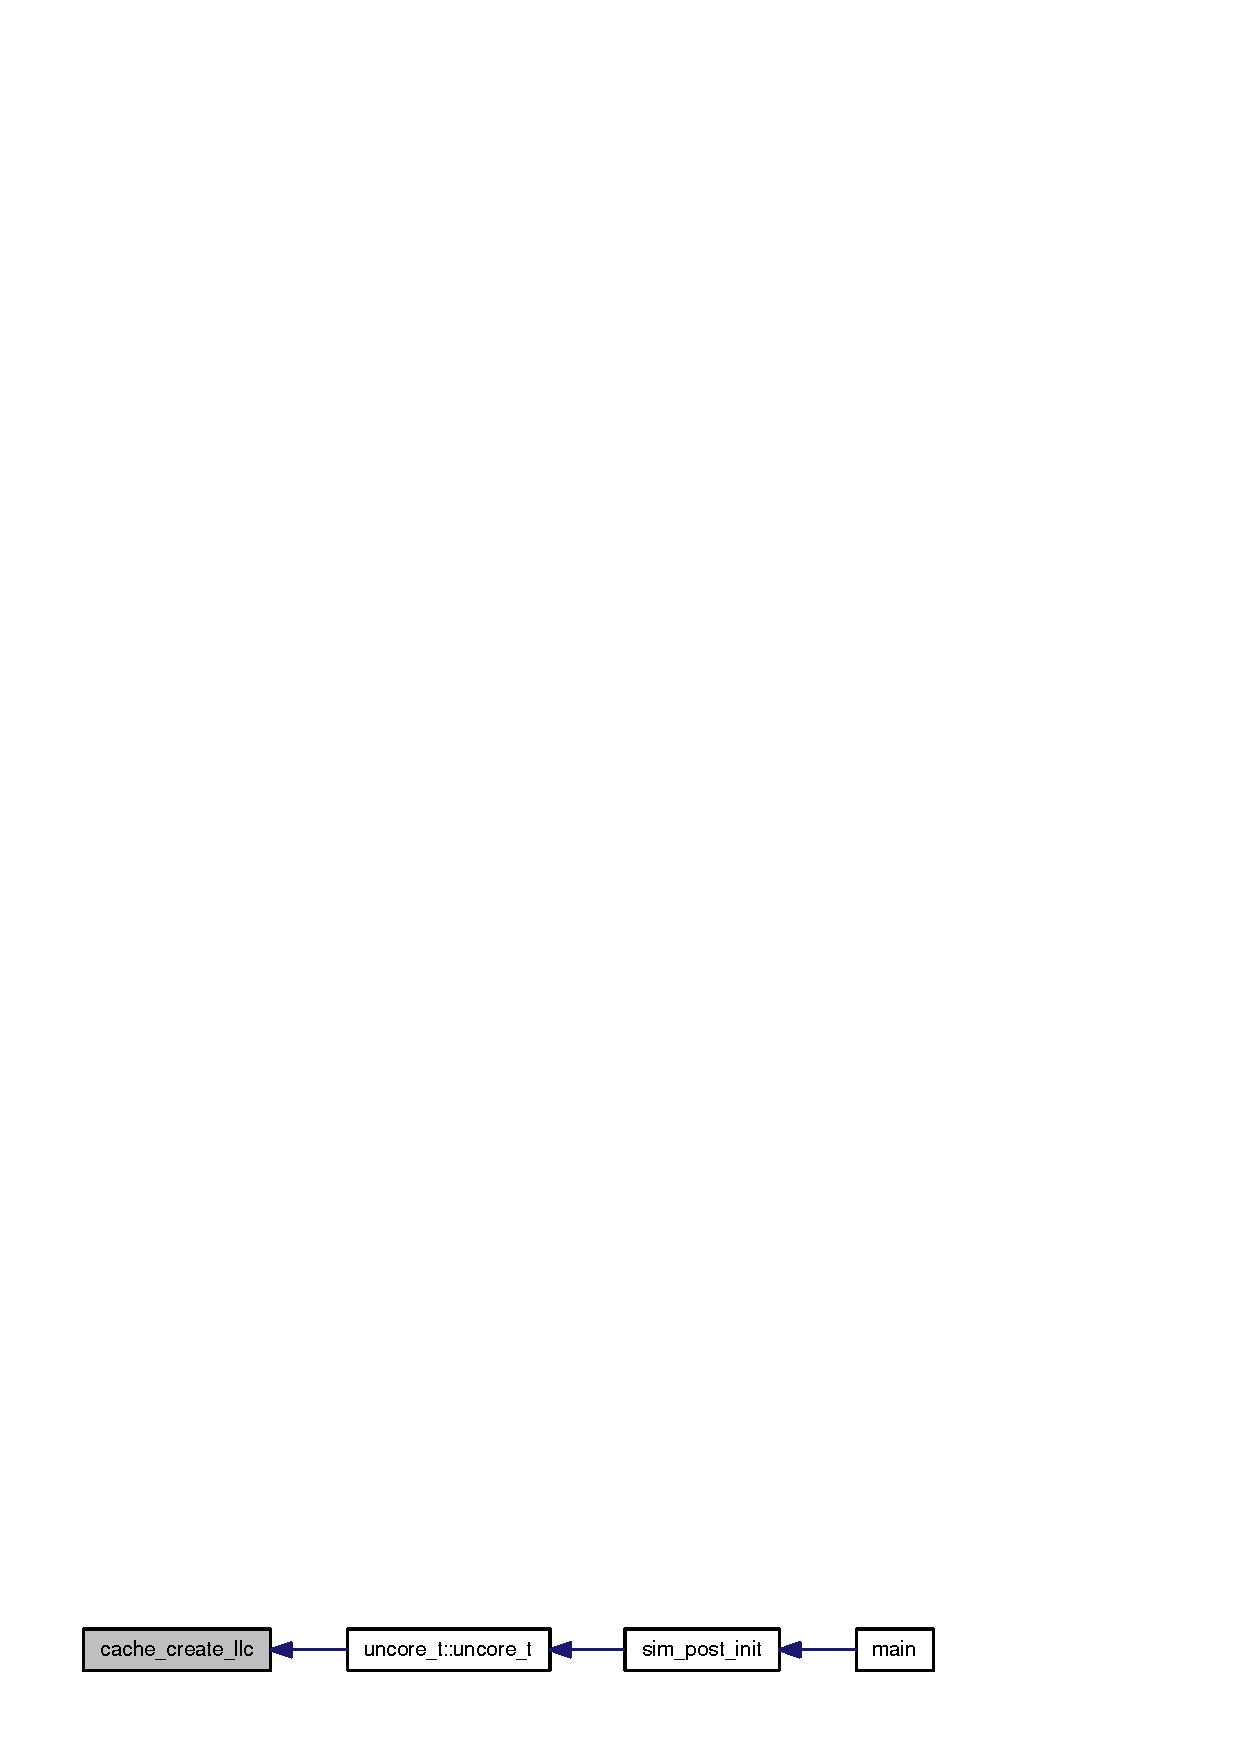
\includegraphics[width=226pt]{zesto-llc_8cpp_727c4cbf039edb120fe825803e69067f_icgraph}
\end{center}
\end{figure}
\index{zesto-llc.cpp@{zesto-llc.cpp}!cache\_\-enqueuable\_\-llc@{cache\_\-enqueuable\_\-llc}}
\index{cache\_\-enqueuable\_\-llc@{cache\_\-enqueuable\_\-llc}!zesto-llc.cpp@{zesto-llc.cpp}}
\subsubsection[{cache\_\-enqueuable\_\-llc}]{\setlength{\rightskip}{0pt plus 5cm}int cache\_\-enqueuable\_\-llc (const struct {\bf cache\_\-t} $\ast$const  {\em cp}, \/  const int {\em thread\_\-id}, \/  const {\bf md\_\-paddr\_\-t} {\em addr})}\label{zesto-llc_8cpp_17919e2800a0393570b40f08156cb42c}




Definition at line 993 of file zesto-llc.cpp.

References DO\_\-NOT\_\-TRANSLATE, GET\_\-BANK, cache\_\-t::latency, and cache\_\-t::pipe\_\-num.

Referenced by cache\_\-process().

Here is the caller graph for this function:\nopagebreak
\begin{figure}[H]
\begin{center}
\leavevmode
\includegraphics[width=232pt]{zesto-llc_8cpp_17919e2800a0393570b40f08156cb42c_icgraph}
\end{center}
\end{figure}
\index{zesto-llc.cpp@{zesto-llc.cpp}!cache\_\-enqueue\_\-llc@{cache\_\-enqueue\_\-llc}}
\index{cache\_\-enqueue\_\-llc@{cache\_\-enqueue\_\-llc}!zesto-llc.cpp@{zesto-llc.cpp}}
\subsubsection[{cache\_\-enqueue\_\-llc}]{\setlength{\rightskip}{0pt plus 5cm}void cache\_\-enqueue\_\-llc (struct {\bf core\_\-t} $\ast$const  {\em core}, \/  struct {\bf cache\_\-t} $\ast$const  {\em cp}, \/  struct {\bf cache\_\-t} $\ast$const  {\em prev\_\-cp}, \/  const enum {\bf cache\_\-command} {\em cmd}, \/  const int {\em thread\_\-id}, \/  const {\bf md\_\-addr\_\-t} {\em PC}, \/  const {\bf md\_\-paddr\_\-t} {\em addr}, \/  const {\bf seq\_\-t} {\em action\_\-id}, \/  const int {\em MSHR\_\-bank}, \/  const int {\em MSHR\_\-index}, \/  void $\ast$const  {\em op}, \/  void($\ast$)(void $\ast$) {\em cb}, \/  void($\ast$)(void $\ast$, int) {\em miss\_\-cb}, \/  bool($\ast$)(void $\ast$, {\bf seq\_\-t}) {\em translated\_\-cb}, \/  {\bf seq\_\-t}($\ast$)(void $\ast$) {\em get\_\-action\_\-id})}\label{zesto-llc_8cpp_6955e78ccb0fb1511754e8cd113e1dcc}




Definition at line 1012 of file zesto-llc.cpp.

References cache\_\-action\_\-t::action\_\-id, cache\_\-assert, cache\_\-heap\_\-balance(), cache\_\-action\_\-t::cb, cache\_\-t::check\_\-for\_\-pipe\_\-work, cache\_\-t::check\_\-for\_\-work, cache\_\-action\_\-t::cmd, cache\_\-action\_\-t::core, DO\_\-NOT\_\-TRANSLATE, cache\_\-action\_\-t::get\_\-action\_\-id, GET\_\-BANK, cache\_\-t::latency, cache\_\-action\_\-t::miss\_\-cb, cache\_\-action\_\-t::miss\_\-cb\_\-invoked, cache\_\-action\_\-t::MSHR\_\-bank, cache\_\-action\_\-t::MSHR\_\-index, cache\_\-action\_\-t::op, cache\_\-action\_\-t::paddr, cache\_\-action\_\-t::PC, cache\_\-t::pipe, cache\_\-action\_\-t::pipe\_\-exit\_\-time, cache\_\-t::pipe\_\-num, cache\_\-action\_\-t::prev\_\-cp, sim\_\-cycle, TICK\_\-T\_\-MAX, cache\_\-action\_\-t::translated\_\-cb, cache\_\-action\_\-t::when\_\-returned, and cache\_\-action\_\-t::when\_\-started.

Referenced by cache\_\-process().

Here is the caller graph for this function:\nopagebreak
\begin{figure}[H]
\begin{center}
\leavevmode
\includegraphics[width=226pt]{zesto-llc_8cpp_6955e78ccb0fb1511754e8cd113e1dcc_icgraph}
\end{center}
\end{figure}
\index{zesto-llc.cpp@{zesto-llc.cpp}!cache\_\-fill\_\-llc@{cache\_\-fill\_\-llc}}
\index{cache\_\-fill\_\-llc@{cache\_\-fill\_\-llc}!zesto-llc.cpp@{zesto-llc.cpp}}
\subsubsection[{cache\_\-fill\_\-llc}]{\setlength{\rightskip}{0pt plus 5cm}static void cache\_\-fill\_\-llc (struct {\bf cache\_\-t} $\ast$const  {\em cp}, \/  const enum {\bf cache\_\-command} {\em cmd}, \/  const {\bf md\_\-paddr\_\-t} {\em paddr}, \/  struct {\bf core\_\-t} $\ast$ {\em core})\hspace{0.3cm}{\tt  [inline, static]}}\label{zesto-llc_8cpp_acfad7c90ec1f20c91ccfcae11d67dea}




Definition at line 1396 of file zesto-llc.cpp.

References cache\_\-assert, cache\_\-t::check\_\-for\_\-fill\_\-work, cache\_\-t::check\_\-for\_\-work, cache\_\-fill\_\-t::cmd, cache\_\-fill\_\-t::core, fill\_\-heap\_\-balance(), cache\_\-t::fill\_\-num, cache\_\-t::fill\_\-pipe, GET\_\-BANK, cache\_\-t::latency, cache\_\-fill\_\-t::paddr, cache\_\-fill\_\-t::pipe\_\-exit\_\-time, sim\_\-cycle, and cache\_\-fill\_\-t::valid.\index{zesto-llc.cpp@{zesto-llc.cpp}!cache\_\-fillable\_\-llc@{cache\_\-fillable\_\-llc}}
\index{cache\_\-fillable\_\-llc@{cache\_\-fillable\_\-llc}!zesto-llc.cpp@{zesto-llc.cpp}}
\subsubsection[{cache\_\-fillable\_\-llc}]{\setlength{\rightskip}{0pt plus 5cm}static bool cache\_\-fillable\_\-llc (const struct {\bf cache\_\-t} $\ast$const  {\em cp}, \/  const {\bf md\_\-paddr\_\-t} {\em paddr})\hspace{0.3cm}{\tt  [inline, static]}}\label{zesto-llc_8cpp_9c38467a1f69e44fd7487395ba6ff279}




Definition at line 1384 of file zesto-llc.cpp.

References cache\_\-t::fill\_\-num, GET\_\-BANK, and cache\_\-t::latency.\index{zesto-llc.cpp@{zesto-llc.cpp}!cache\_\-get\_\-evictee\_\-llc@{cache\_\-get\_\-evictee\_\-llc}}
\index{cache\_\-get\_\-evictee\_\-llc@{cache\_\-get\_\-evictee\_\-llc}!zesto-llc.cpp@{zesto-llc.cpp}}
\subsubsection[{cache\_\-get\_\-evictee\_\-llc}]{\setlength{\rightskip}{0pt plus 5cm}struct {\bf cache\_\-line\_\-t}$\ast$ cache\_\-get\_\-evictee\_\-llc (struct {\bf cache\_\-t} $\ast$const  {\em cp}, \/  const {\bf md\_\-paddr\_\-t} {\em addr}, \/  {\bf core\_\-t} $\ast$const  {\em core})\hspace{0.3cm}{\tt  [read]}}\label{zesto-llc_8cpp_edb31cd34331b82f67b46e4117a3fb7a}




Definition at line 755 of file zesto-llc.cpp.

References cache\_\-t::addr\_\-shift, cache\_\-t::assoc, cache\_\-t::blocks, fatal(), cache\_\-t::log2\_\-assoc, cache\_\-line\_\-t::meta, modinc(), cache\_\-t::name, cache\_\-line\_\-t::next, REPLACE\_\-CLOCK, REPLACE\_\-LRU, REPLACE\_\-MRU, REPLACE\_\-NMRU, REPLACE\_\-PLRU, REPLACE\_\-RANDOM, cache\_\-t::replacement\_\-policy, cache\_\-t::sets, cache\_\-line\_\-t::valid, and cache\_\-line\_\-t::way.

Referenced by cache\_\-process\_\-llc(), and sim\_\-fastfwd().

Here is the caller graph for this function:\nopagebreak
\begin{figure}[H]
\begin{center}
\leavevmode
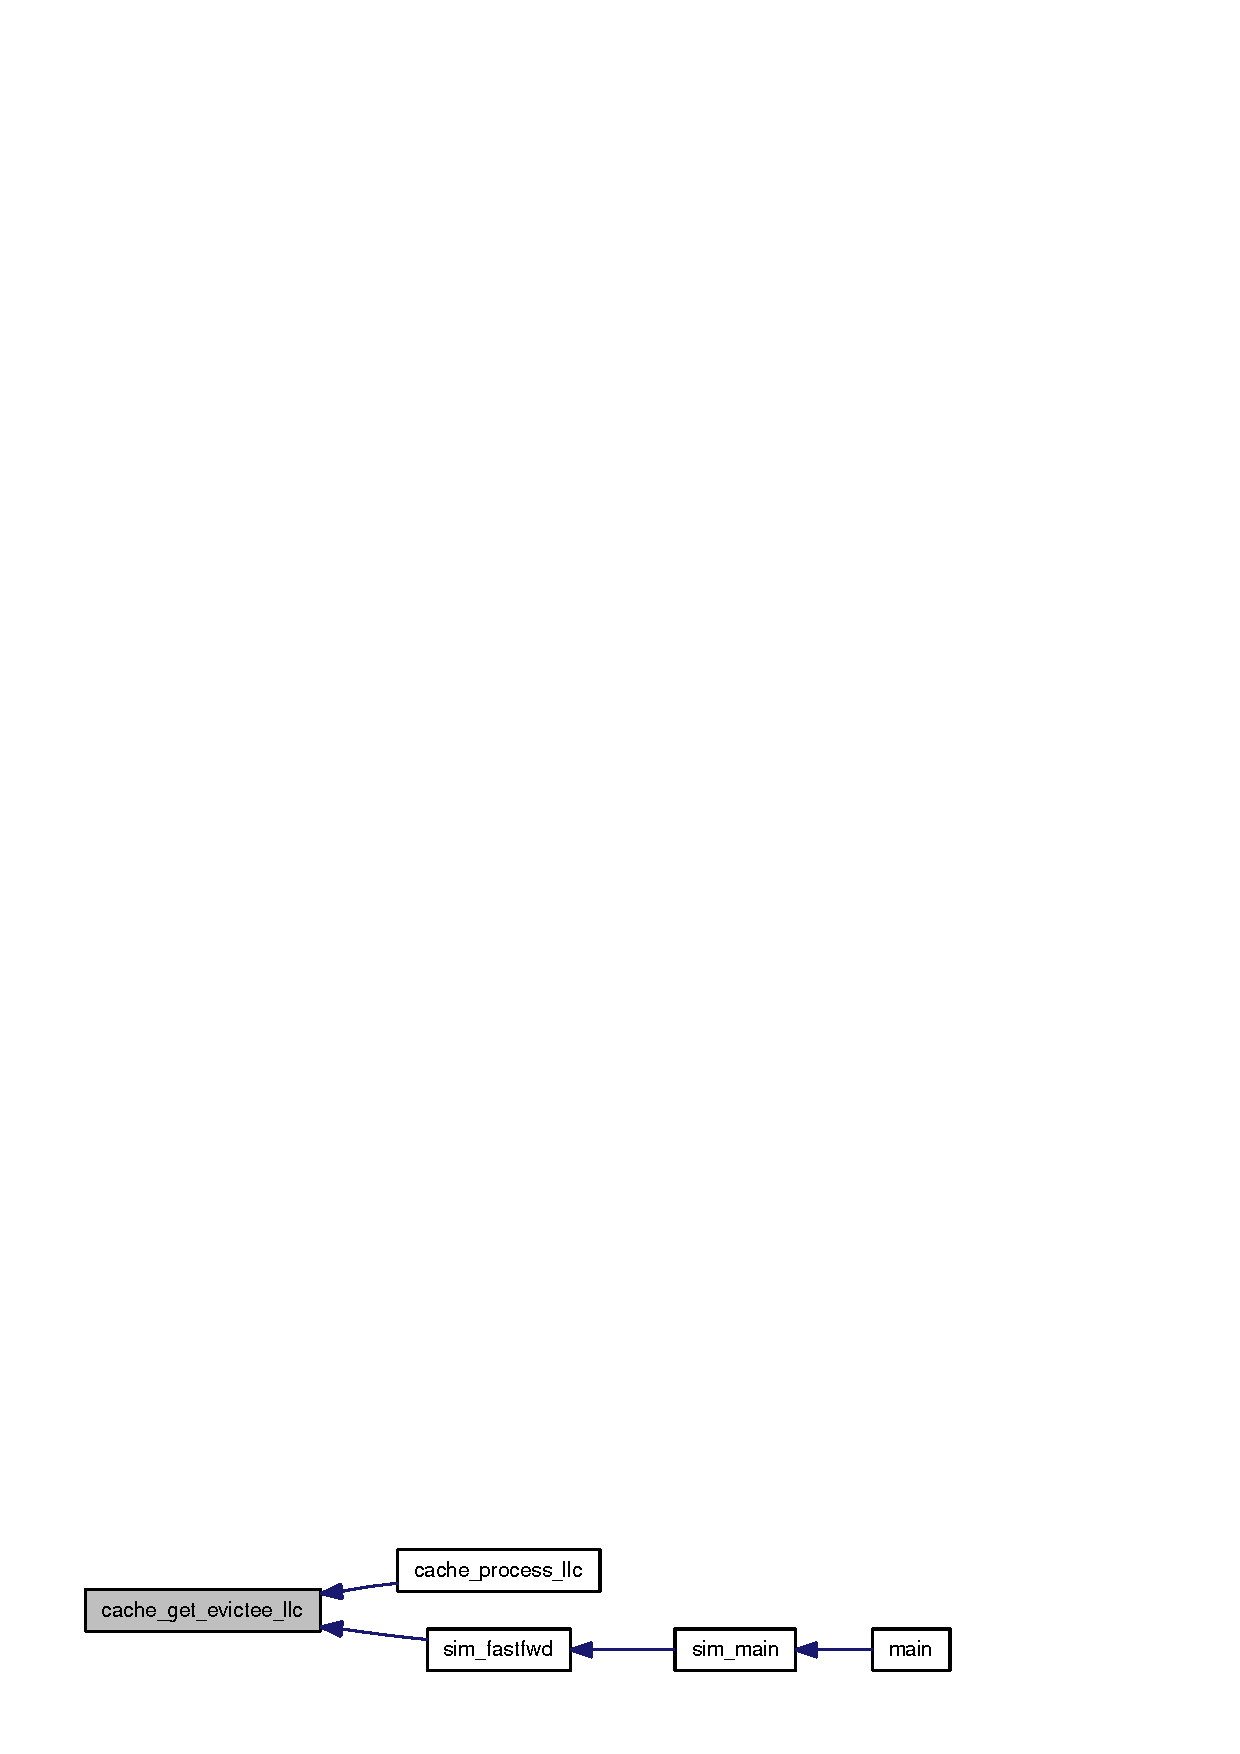
\includegraphics[width=230pt]{zesto-llc_8cpp_edb31cd34331b82f67b46e4117a3fb7a_icgraph}
\end{center}
\end{figure}
\index{zesto-llc.cpp@{zesto-llc.cpp}!cache\_\-heap\_\-balance@{cache\_\-heap\_\-balance}}
\index{cache\_\-heap\_\-balance@{cache\_\-heap\_\-balance}!zesto-llc.cpp@{zesto-llc.cpp}}
\subsubsection[{cache\_\-heap\_\-balance}]{\setlength{\rightskip}{0pt plus 5cm}static void cache\_\-heap\_\-balance (struct {\bf cache\_\-action\_\-t} $\ast$const  {\em pipe}, \/  const int {\em insert\_\-position})\hspace{0.3cm}{\tt  [static]}}\label{zesto-llc_8cpp_0784d914ca0e1dc0f651a456830f94ed}




Definition at line 897 of file zesto-llc.cpp.

References memswap().\index{zesto-llc.cpp@{zesto-llc.cpp}!cache\_\-heap\_\-remove@{cache\_\-heap\_\-remove}}
\index{cache\_\-heap\_\-remove@{cache\_\-heap\_\-remove}!zesto-llc.cpp@{zesto-llc.cpp}}
\subsubsection[{cache\_\-heap\_\-remove}]{\setlength{\rightskip}{0pt plus 5cm}static void cache\_\-heap\_\-remove (struct {\bf cache\_\-action\_\-t} $\ast$const  {\em pipe}, \/  const int {\em pipe\_\-num})\hspace{0.3cm}{\tt  [static]}}\label{zesto-llc_8cpp_672e06f81a893ac6af2c4fd4948069ed}




Definition at line 923 of file zesto-llc.cpp.

References cache\_\-action\_\-t::cb, memswap(), cache\_\-action\_\-t::pipe\_\-exit\_\-time, and TICK\_\-T\_\-MAX.\index{zesto-llc.cpp@{zesto-llc.cpp}!cache\_\-insert\_\-block\_\-llc@{cache\_\-insert\_\-block\_\-llc}}
\index{cache\_\-insert\_\-block\_\-llc@{cache\_\-insert\_\-block\_\-llc}!zesto-llc.cpp@{zesto-llc.cpp}}
\subsubsection[{cache\_\-insert\_\-block\_\-llc}]{\setlength{\rightskip}{0pt plus 5cm}void cache\_\-insert\_\-block\_\-llc (struct {\bf cache\_\-t} $\ast$const  {\em cp}, \/  const enum {\bf cache\_\-command} {\em cmd}, \/  const {\bf md\_\-paddr\_\-t} {\em addr}, \/  {\bf core\_\-t} $\ast$const  {\em core})}\label{zesto-llc_8cpp_e7c14fa8601433a16fa1cd5f91e64c7c}




Definition at line 656 of file zesto-llc.cpp.

References cache\_\-t::addr\_\-shift, cache\_\-t::blocks, cache\_\-assert, CACHE\_\-PREFETCH, CACHE\_\-STAT, CACHE\_\-WRITE, CACHE\_\-WRITEBACK, cache\_\-line\_\-t::core, cache\_\-line\_\-t::dirty, fatal(), cache\_\-t::log2\_\-assoc, cache\_\-line\_\-t::meta, cache\_\-line\_\-t::next, cache\_\-t::prefetch\_\-insertions, cache\_\-line\_\-t::prefetched, REPLACE\_\-CLOCK, REPLACE\_\-LRU, REPLACE\_\-MRU, REPLACE\_\-NMRU, REPLACE\_\-PLRU, REPLACE\_\-RANDOM, cache\_\-t::replacement\_\-policy, cache\_\-t::sets, cache\_\-t::stat, cache\_\-line\_\-t::tag, cache\_\-line\_\-t::valid, and cache\_\-line\_\-t::way.

Referenced by cache\_\-process\_\-llc(), and sim\_\-fastfwd().

Here is the caller graph for this function:\nopagebreak
\begin{figure}[H]
\begin{center}
\leavevmode
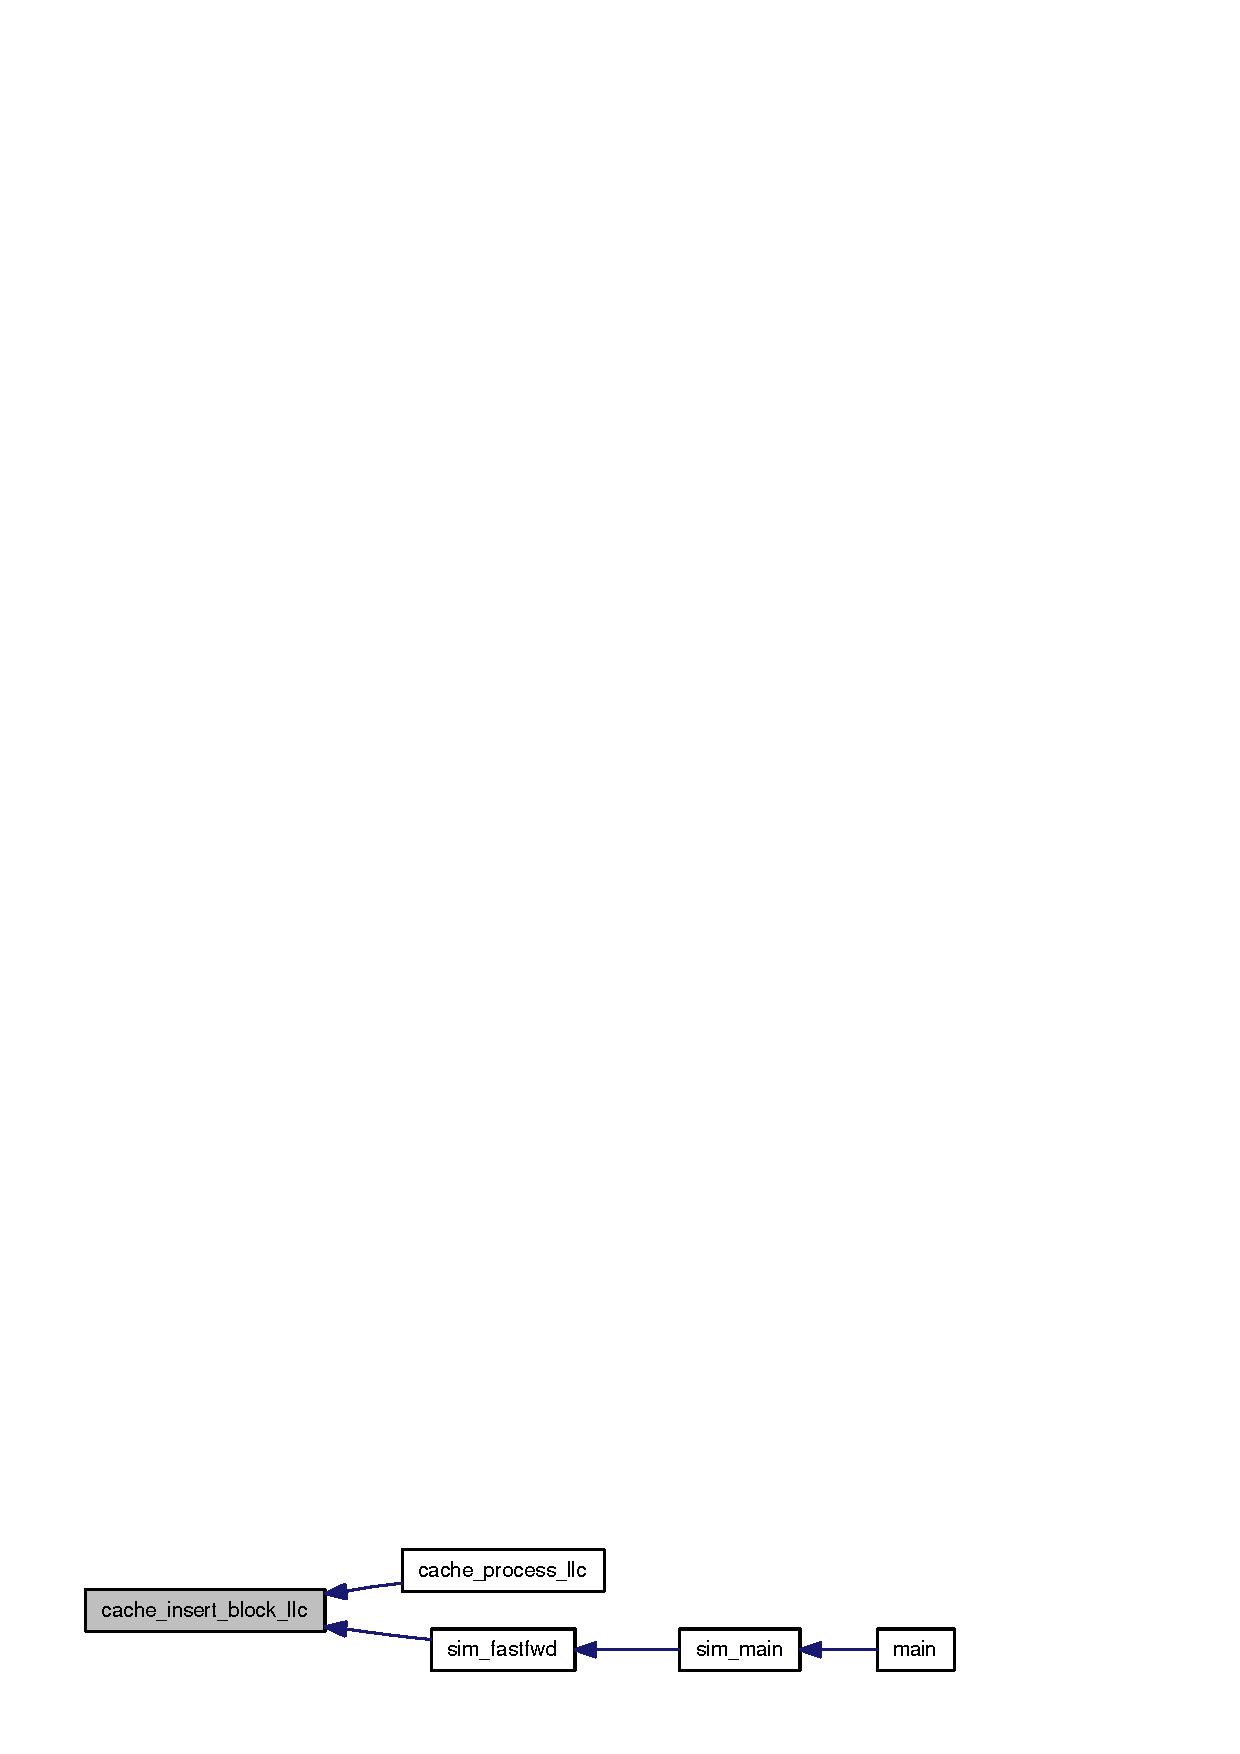
\includegraphics[width=231pt]{zesto-llc_8cpp_e7c14fa8601433a16fa1cd5f91e64c7c_icgraph}
\end{center}
\end{figure}
\index{zesto-llc.cpp@{zesto-llc.cpp}!cache\_\-is\_\-hit\_\-llc@{cache\_\-is\_\-hit\_\-llc}}
\index{cache\_\-is\_\-hit\_\-llc@{cache\_\-is\_\-hit\_\-llc}!zesto-llc.cpp@{zesto-llc.cpp}}
\subsubsection[{cache\_\-is\_\-hit\_\-llc}]{\setlength{\rightskip}{0pt plus 5cm}struct {\bf cache\_\-line\_\-t}$\ast$ cache\_\-is\_\-hit\_\-llc (struct {\bf cache\_\-t} $\ast$const  {\em cp}, \/  const enum {\bf cache\_\-command} {\em cmd}, \/  const {\bf md\_\-paddr\_\-t} {\em addr}, \/  struct {\bf core\_\-t} $\ast$const  {\em core})\hspace{0.3cm}{\tt  [read]}}\label{zesto-llc_8cpp_4c8a74cb2e996679500e5a9adb9efb5c}




Definition at line 532 of file zesto-llc.cpp.

References cache\_\-t::addr\_\-shift, cache\_\-t::blocks, cache\_\-assert, CACHE\_\-READONLY, CACHE\_\-WRITE, CACHE\_\-WRITEBACK, cache\_\-line\_\-t::dirty, fatal(), cache\_\-t::log2\_\-assoc, cache\_\-line\_\-t::meta, cache\_\-line\_\-t::next, cache\_\-t::read\_\-only, REPLACE\_\-CLOCK, REPLACE\_\-LRU, REPLACE\_\-MRU, REPLACE\_\-NMRU, REPLACE\_\-PLRU, REPLACE\_\-RANDOM, cache\_\-t::replacement\_\-policy, cache\_\-t::sets, cache\_\-line\_\-t::tag, cache\_\-line\_\-t::valid, cache\_\-line\_\-t::way, WRITE\_\-BACK, and cache\_\-t::write\_\-policy.

Referenced by cache\_\-process\_\-llc(), and sim\_\-fastfwd().

Here is the caller graph for this function:\nopagebreak
\begin{figure}[H]
\begin{center}
\leavevmode
\includegraphics[width=216pt]{zesto-llc_8cpp_4c8a74cb2e996679500e5a9adb9efb5c_icgraph}
\end{center}
\end{figure}
\index{zesto-llc.cpp@{zesto-llc.cpp}!cache\_\-peek\_\-llc@{cache\_\-peek\_\-llc}}
\index{cache\_\-peek\_\-llc@{cache\_\-peek\_\-llc}!zesto-llc.cpp@{zesto-llc.cpp}}
\subsubsection[{cache\_\-peek\_\-llc}]{\setlength{\rightskip}{0pt plus 5cm}static struct {\bf cache\_\-line\_\-t}$\ast$ cache\_\-peek\_\-llc (const struct {\bf cache\_\-t} $\ast$const  {\em cp}, \/  const {\bf md\_\-paddr\_\-t} {\em addr})\hspace{0.3cm}{\tt  [static, read]}}\label{zesto-llc_8cpp_955da6a438bbb3f390d758f2f75fa822}




Definition at line 631 of file zesto-llc.cpp.

References cache\_\-t::addr\_\-shift, cache\_\-t::blocks, cache\_\-line\_\-t::next, cache\_\-t::sets, cache\_\-line\_\-t::tag, and cache\_\-line\_\-t::valid.\index{zesto-llc.cpp@{zesto-llc.cpp}!cache\_\-prefetch\_\-llc@{cache\_\-prefetch\_\-llc}}
\index{cache\_\-prefetch\_\-llc@{cache\_\-prefetch\_\-llc}!zesto-llc.cpp@{zesto-llc.cpp}}
\subsubsection[{cache\_\-prefetch\_\-llc}]{\setlength{\rightskip}{0pt plus 5cm}static void cache\_\-prefetch\_\-llc (struct {\bf cache\_\-t} $\ast$const  {\em cp})\hspace{0.3cm}{\tt  [static]}}\label{zesto-llc_8cpp_0bb0f060c77b60c70dce0eee1abb237a}




Definition at line 2130 of file zesto-llc.cpp.

References cache\_\-t::cache\_\-t::PFF\_\-t::addr, cache\_\-assert, cache\_\-enqueuable(), cache\_\-enqueue(), CACHE\_\-PREFETCH, cache\_\-t::cache\_\-t::PFF\_\-t::core, DO\_\-NOT\_\-TRANSLATE, dummy\_\-callback(), GET\_\-MSHR\_\-BANK, modinc(), NO\_\-MSHR, cache\_\-t::cache\_\-t::PFF\_\-t::PC, PF\_\-OK, cache\_\-t::PF\_\-sample\_\-interval, cache\_\-t::PF\_\-state, cache\_\-t::PFF, cache\_\-t::PFF\_\-head, cache\_\-t::PFF\_\-num, cache\_\-t::PFF\_\-size, cache\_\-t::prefetch\_\-max, and cache\_\-t::prefetch\_\-threshold.\index{zesto-llc.cpp@{zesto-llc.cpp}!cache\_\-process\_\-llc@{cache\_\-process\_\-llc}}
\index{cache\_\-process\_\-llc@{cache\_\-process\_\-llc}!zesto-llc.cpp@{zesto-llc.cpp}}
\subsubsection[{cache\_\-process\_\-llc}]{\setlength{\rightskip}{0pt plus 5cm}void cache\_\-process\_\-llc (struct {\bf cache\_\-t} $\ast$const  {\em cp})}\label{zesto-llc_8cpp_7b2967a29a17913e313fceec0d9dbd4c}




Definition at line 1427 of file zesto-llc.cpp.

References cache\_\-action\_\-t::action\_\-id, cache\_\-t::cache\_\-t::PFF\_\-t::addr, prefetch\_\-buffer\_\-t::addr, cache\_\-t::addr\_\-shift, cache\_\-t::allocate\_\-policy, cache\_\-t::bank\_\-mask, cache\_\-t::banks, BIG\_\-LATENCY, bus\_\-free(), bus\_\-use(), cache\_\-assert, cache\_\-fill\_\-llc(), cache\_\-fillable\_\-llc(), cache\_\-get\_\-evictee\_\-llc(), cache\_\-heap\_\-remove(), cache\_\-insert\_\-block\_\-llc(), cache\_\-invalidate(), cache\_\-is\_\-hit\_\-llc(), cache\_\-peek\_\-llc(), CACHE\_\-PREFETCH, CACHE\_\-READ, CACHE\_\-STAT, CACHE\_\-WRITE, CACHE\_\-WRITEBACK, cache\_\-action\_\-t::cb, cache\_\-t::check\_\-for\_\-fill\_\-work, cache\_\-t::check\_\-for\_\-MSHR\_\-fill\_\-work, cache\_\-t::check\_\-for\_\-MSHR\_\-work, cache\_\-t::check\_\-for\_\-pipe\_\-work, cache\_\-t::check\_\-for\_\-WBB\_\-work, cache\_\-t::check\_\-for\_\-work, cache\_\-action\_\-t::cmd, cache\_\-t::cache\_\-t::PFF\_\-t::core, cache\_\-line\_\-t::core, cache\_\-t::core, cache\_\-action\_\-t::core, cache\_\-t::core\_\-lookups, cache\_\-t::core\_\-misses, cache\_\-line\_\-t::dirty, uncore\_\-t::enqueuable(), uncore\_\-t::enqueue(), fatal(), fill\_\-arrived(), fill\_\-heap\_\-remove(), cache\_\-t::fill\_\-num, cache\_\-t::fill\_\-pipe, cache\_\-action\_\-t::get\_\-action\_\-id, GET\_\-MSHR\_\-BANK, cache\_\-t::latency, cache\_\-t::linesize, uncore\_\-t::LLC, cache\_\-t::load\_\-lookups, cache\_\-t::load\_\-misses, prefetch\_\-t::lookup(), cache\_\-action\_\-t::miss\_\-cb, cache\_\-action\_\-t::miss\_\-cb\_\-invoked, modinc(), cache\_\-t::MSHR, MSHR\_\-allocate(), MSHR\_\-available(), cache\_\-action\_\-t::MSHR\_\-bank, cache\_\-t::MSHR\_\-banks, cache\_\-t::MSHR\_\-full\_\-cycles, cache\_\-action\_\-t::MSHR\_\-index, cache\_\-action\_\-t::MSHR\_\-linked, cache\_\-t::MSHR\_\-mask, cache\_\-t::MSHR\_\-occupancy, cache\_\-t::MSHR\_\-size, cache\_\-t::name, prefetch\_\-buffer\_\-t::next, cache\_\-t::next\_\-bus, cache\_\-t::next\_\-level, NO\_\-MSHR, cache\_\-t::num\_\-prefetchers, cache\_\-action\_\-t::op, cache\_\-action\_\-t::paddr, PAGE\_\-SIZE, cache\_\-t::cache\_\-t::PFF\_\-t::PC, cache\_\-t::PF\_\-buffer, cache\_\-t::PF\_\-filter, cache\_\-t::PFF, cache\_\-t::PFF\_\-head, cache\_\-t::PFF\_\-num, cache\_\-t::PFF\_\-size, cache\_\-t::PFF\_\-tail, cache\_\-t::pipe, cache\_\-t::pipe\_\-num, prefetch\_\-filter\_\-lookup(), prefetch\_\-filter\_\-update(), cache\_\-t::prefetch\_\-lookups, cache\_\-t::prefetch\_\-misses, cache\_\-t::prefetch\_\-on\_\-miss, cache\_\-line\_\-t::prefetch\_\-used, cache\_\-t::prefetch\_\-useful\_\-insertions, cache\_\-line\_\-t::prefetched, cache\_\-t::prefetcher, cache\_\-action\_\-t::prev\_\-cp, cache\_\-t::prev\_\-level, sim\_\-cycle, cache\_\-t::start\_\-point, cache\_\-t::stat, cache\_\-t::store\_\-lookups, cache\_\-t::store\_\-misses, cache\_\-line\_\-t::tag, TICK\_\-T\_\-MAX, cache\_\-action\_\-t::translated\_\-cb, cache\_\-t::uncore, cache\_\-line\_\-t::valid, cache\_\-line\_\-t::victim, cache\_\-t::WBB, WBB\_\-available(), cache\_\-t::WBB\_\-combines, cache\_\-t::WBB\_\-full\_\-cycles, cache\_\-t::WBB\_\-head, cache\_\-t::WBB\_\-hits, WBB\_\-insert(), cache\_\-t::WBB\_\-num, cache\_\-t::WBB\_\-occupancy, cache\_\-t::WBB\_\-size, cache\_\-t::WBB\_\-victim\_\-hits, cache\_\-action\_\-t::when\_\-enqueued, cache\_\-action\_\-t::when\_\-returned, cache\_\-action\_\-t::when\_\-started, WRITE\_\-ALLOC, WRITE\_\-BACK, cache\_\-t::write\_\-combining, cache\_\-t::write\_\-policy, WRITE\_\-THROUGH, cache\_\-t::writeback\_\-lookups, and cache\_\-t::writeback\_\-misses.

Referenced by zesto\_\-component::downtick\_\-handler().

Here is the caller graph for this function:\nopagebreak
\begin{figure}[H]
\begin{center}
\leavevmode
\includegraphics[width=320pt]{zesto-llc_8cpp_7b2967a29a17913e313fceec0d9dbd4c_icgraph}
\end{center}
\end{figure}
\index{zesto-llc.cpp@{zesto-llc.cpp}!dummy\_\-callback@{dummy\_\-callback}}
\index{dummy\_\-callback@{dummy\_\-callback}!zesto-llc.cpp@{zesto-llc.cpp}}
\subsubsection[{dummy\_\-callback}]{\setlength{\rightskip}{0pt plus 5cm}static void dummy\_\-callback (void $\ast$ {\em p})\hspace{0.3cm}{\tt  [static]}}\label{zesto-llc_8cpp_2ca1ae8eb0053c08276d5e170a5f98d8}




Definition at line 1243 of file zesto-llc.cpp.\index{zesto-llc.cpp@{zesto-llc.cpp}!fill\_\-arrived\_\-llc@{fill\_\-arrived\_\-llc}}
\index{fill\_\-arrived\_\-llc@{fill\_\-arrived\_\-llc}!zesto-llc.cpp@{zesto-llc.cpp}}
\subsubsection[{fill\_\-arrived\_\-llc}]{\setlength{\rightskip}{0pt plus 5cm}void fill\_\-arrived\_\-llc (struct {\bf cache\_\-t} $\ast$const  {\em cp}, \/  unsigned long long int {\em address})}\label{zesto-llc_8cpp_f1f903df28f067bfd63f3145c04a5870}




Definition at line 1250 of file zesto-llc.cpp.

References cache\_\-t::addr\_\-shift, cache\_\-action\_\-t::cb, cache\_\-t::check\_\-for\_\-MSHR\_\-fill\_\-work, cache\_\-t::check\_\-for\_\-work, cache\_\-t::MSHR, cache\_\-t::MSHR\_\-banks, cache\_\-action\_\-t::MSHR\_\-link, cache\_\-action\_\-t::MSHR\_\-linked, cache\_\-t::MSHR\_\-mask, cache\_\-t::MSHR\_\-size, cache\_\-action\_\-t::paddr, sim\_\-cycle, and cache\_\-action\_\-t::when\_\-returned.

Referenced by uncore\_\-t::handle\_\-new\_\-packet\_\-event().

Here is the caller graph for this function:\nopagebreak
\begin{figure}[H]
\begin{center}
\leavevmode
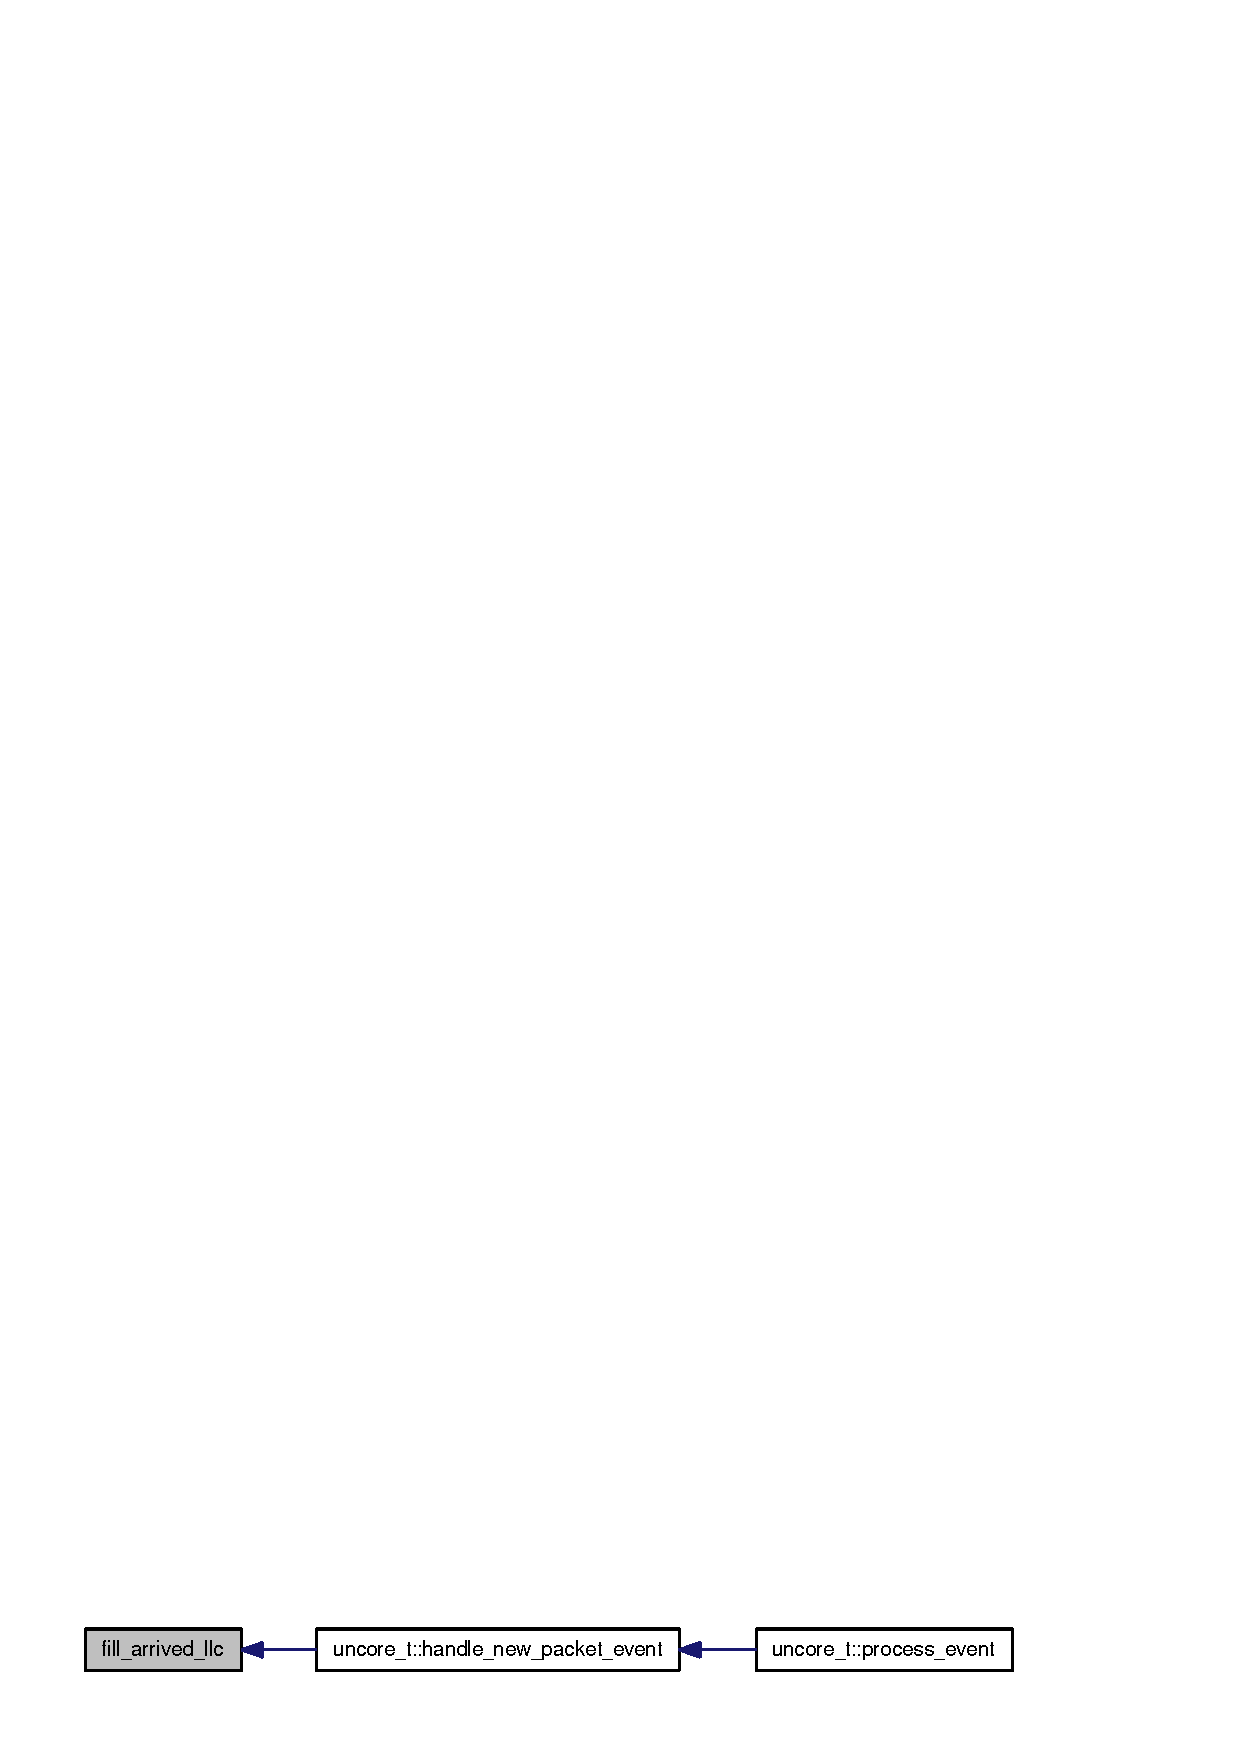
\includegraphics[width=245pt]{zesto-llc_8cpp_f1f903df28f067bfd63f3145c04a5870_icgraph}
\end{center}
\end{figure}
\index{zesto-llc.cpp@{zesto-llc.cpp}!fill\_\-heap\_\-balance@{fill\_\-heap\_\-balance}}
\index{fill\_\-heap\_\-balance@{fill\_\-heap\_\-balance}!zesto-llc.cpp@{zesto-llc.cpp}}
\subsubsection[{fill\_\-heap\_\-balance}]{\setlength{\rightskip}{0pt plus 5cm}static void fill\_\-heap\_\-balance (struct {\bf cache\_\-fill\_\-t} $\ast$const  {\em pipe}, \/  const int {\em insert\_\-position})\hspace{0.3cm}{\tt  [static]}}\label{zesto-llc_8cpp_45008d7fc6cedc3c5187a70e4cfc1d4a}




Definition at line 1291 of file zesto-llc.cpp.

References memswap(), and cache\_\-action\_\-t::pipe\_\-exit\_\-time.\index{zesto-llc.cpp@{zesto-llc.cpp}!fill\_\-heap\_\-remove@{fill\_\-heap\_\-remove}}
\index{fill\_\-heap\_\-remove@{fill\_\-heap\_\-remove}!zesto-llc.cpp@{zesto-llc.cpp}}
\subsubsection[{fill\_\-heap\_\-remove}]{\setlength{\rightskip}{0pt plus 5cm}static void fill\_\-heap\_\-remove (struct {\bf cache\_\-fill\_\-t} $\ast$const  {\em pipe}, \/  const int {\em pipe\_\-num})\hspace{0.3cm}{\tt  [static]}}\label{zesto-llc_8cpp_9c8931eb6f26a4862221d39dd688368f}




Definition at line 1315 of file zesto-llc.cpp.

References memswap(), cache\_\-fill\_\-t::pipe\_\-exit\_\-time, TICK\_\-T\_\-MAX, and cache\_\-fill\_\-t::valid.\index{zesto-llc.cpp@{zesto-llc.cpp}!LLC\_\-reg\_\-stats@{LLC\_\-reg\_\-stats}}
\index{LLC\_\-reg\_\-stats@{LLC\_\-reg\_\-stats}!zesto-llc.cpp@{zesto-llc.cpp}}
\subsubsection[{LLC\_\-reg\_\-stats}]{\setlength{\rightskip}{0pt plus 5cm}void LLC\_\-reg\_\-stats (struct {\bf stat\_\-sdb\_\-t} $\ast$const  {\em sdb}, \/  struct {\bf cache\_\-t} $\ast$const  {\em cp})}\label{zesto-llc_8cpp_0a1aa47236ccba0a1d5e5818052a830d}




Definition at line 284 of file zesto-llc.cpp.

References CACHE\_\-READWRITE, uncore\_\-t::core, cache\_\-t::core\_\-lookups, cache\_\-t::core\_\-misses, core\_\-t::id, cache\_\-t::load\_\-lookups, cache\_\-t::load\_\-misses, cache\_\-t::MSHR\_\-combos, cache\_\-t::MSHR\_\-full\_\-cycles, cache\_\-t::MSHR\_\-occupancy, cache\_\-t::name, NetworkComponent::node\_\-ip, uncore\_\-t::num\_\-cores, cache\_\-t::num\_\-prefetchers, num\_\-threads, cache\_\-t::prefetch\_\-insertions, cache\_\-t::prefetch\_\-lookups, cache\_\-t::prefetch\_\-misses, cache\_\-t::prefetch\_\-useful\_\-insertions, cache\_\-t::prefetcher, cache\_\-t::read\_\-only, prefetch\_\-t::reg\_\-stats(), cache\_\-t::stat, stat\_\-reg\_\-counter, stat\_\-reg\_\-formula(), cache\_\-t::store\_\-lookups, cache\_\-t::store\_\-misses, cache\_\-t::uncore, cache\_\-t::WBB\_\-combines, cache\_\-t::WBB\_\-full\_\-cycles, cache\_\-t::WBB\_\-hits, cache\_\-t::WBB\_\-insertions, cache\_\-t::WBB\_\-occupancy, cache\_\-t::WBB\_\-victim\_\-hits, cache\_\-t::WBB\_\-victim\_\-insertions, cache\_\-t::writeback\_\-lookups, and cache\_\-t::writeback\_\-misses.

Referenced by uncore\_\-t::uncore\_\-reg\_\-stats().

Here is the caller graph for this function:\nopagebreak
\begin{figure}[H]
\begin{center}
\leavevmode
\includegraphics[width=147pt]{zesto-llc_8cpp_0a1aa47236ccba0a1d5e5818052a830d_icgraph}
\end{center}
\end{figure}
\index{zesto-llc.cpp@{zesto-llc.cpp}!MSHR\_\-allocate@{MSHR\_\-allocate}}
\index{MSHR\_\-allocate@{MSHR\_\-allocate}!zesto-llc.cpp@{zesto-llc.cpp}}
\subsubsection[{MSHR\_\-allocate}]{\setlength{\rightskip}{0pt plus 5cm}static struct {\bf cache\_\-action\_\-t}$\ast$ MSHR\_\-allocate (struct {\bf cache\_\-t} $\ast$const  {\em cp}, \/  const {\bf md\_\-paddr\_\-t} {\em paddr}, \/  const enum {\bf cache\_\-command} {\em cmd})\hspace{0.3cm}{\tt  [static, read]}}\label{zesto-llc_8cpp_b9e90f1afc77db8eb4dad712b12304ac}




Definition at line 1189 of file zesto-llc.cpp.

References cache\_\-t::addr\_\-shift, cache\_\-assert, cache\_\-action\_\-t::cb, cache\_\-t::check\_\-for\_\-MSHR\_\-work, cache\_\-t::check\_\-for\_\-work, fatal(), GET\_\-MSHR\_\-BANK, cache\_\-t::MSHR, cache\_\-t::MSHR\_\-combos, cache\_\-action\_\-t::MSHR\_\-link, cache\_\-action\_\-t::MSHR\_\-linked, cache\_\-t::MSHR\_\-size, cache\_\-action\_\-t::paddr, cache\_\-t::stat, TICK\_\-T\_\-MAX, and cache\_\-action\_\-t::when\_\-returned.\index{zesto-llc.cpp@{zesto-llc.cpp}!MSHR\_\-available@{MSHR\_\-available}}
\index{MSHR\_\-available@{MSHR\_\-available}!zesto-llc.cpp@{zesto-llc.cpp}}
\subsubsection[{MSHR\_\-available}]{\setlength{\rightskip}{0pt plus 5cm}static int MSHR\_\-available (const struct {\bf cache\_\-t} $\ast$const  {\em cp}, \/  const {\bf md\_\-paddr\_\-t} {\em paddr})\hspace{0.3cm}{\tt  [inline, static]}}\label{zesto-llc_8cpp_eb1b85c3ab5d1ac1520577d21fd09dee}




Definition at line 1179 of file zesto-llc.cpp.

References GET\_\-MSHR\_\-BANK, and cache\_\-t::MSHR\_\-size.\index{zesto-llc.cpp@{zesto-llc.cpp}!prefetch\_\-controller\_\-update\_\-llc@{prefetch\_\-controller\_\-update\_\-llc}}
\index{prefetch\_\-controller\_\-update\_\-llc@{prefetch\_\-controller\_\-update\_\-llc}!zesto-llc.cpp@{zesto-llc.cpp}}
\subsubsection[{prefetch\_\-controller\_\-update\_\-llc}]{\setlength{\rightskip}{0pt plus 5cm}static void prefetch\_\-controller\_\-update\_\-llc (struct {\bf cache\_\-t} $\ast$const  {\em cp})\hspace{0.3cm}{\tt  [static]}}\label{zesto-llc_8cpp_2a67725e0ce33f38cea945ca6beef7d7}




Definition at line 2159 of file zesto-llc.cpp.

References cache\_\-t::PF\_\-high\_\-watermark, cache\_\-t::PF\_\-last\_\-sample, PF\_\-OK, PF\_\-REFRAIN, cache\_\-t::PF\_\-sample\_\-interval, cache\_\-t::PF\_\-state, sim\_\-cycle, cache\_\-t::stat, and cache\_\-t::uncore\_\-utilization.\index{zesto-llc.cpp@{zesto-llc.cpp}!prefetch\_\-filter\_\-lookup@{prefetch\_\-filter\_\-lookup}}
\index{prefetch\_\-filter\_\-lookup@{prefetch\_\-filter\_\-lookup}!zesto-llc.cpp@{zesto-llc.cpp}}
\subsubsection[{prefetch\_\-filter\_\-lookup}]{\setlength{\rightskip}{0pt plus 5cm}static int prefetch\_\-filter\_\-lookup (struct {\bf prefetch\_\-filter\_\-t} $\ast$const  {\em p}, \/  const {\bf md\_\-paddr\_\-t} {\em addr})\hspace{0.3cm}{\tt  [static]}}\label{zesto-llc_8cpp_17dbb4e8d2ae84f22541bef1c04253de}




Definition at line 486 of file zesto-llc.cpp.

References prefetch\_\-filter\_\-t::last\_\-reset, prefetch\_\-filter\_\-t::mask, prefetch\_\-filter\_\-t::num\_\-entries, prefetch\_\-filter\_\-t::reset\_\-interval, sim\_\-cycle, and prefetch\_\-filter\_\-t::table.\index{zesto-llc.cpp@{zesto-llc.cpp}!prefetch\_\-filter\_\-update@{prefetch\_\-filter\_\-update}}
\index{prefetch\_\-filter\_\-update@{prefetch\_\-filter\_\-update}!zesto-llc.cpp@{zesto-llc.cpp}}
\subsubsection[{prefetch\_\-filter\_\-update}]{\setlength{\rightskip}{0pt plus 5cm}static void prefetch\_\-filter\_\-update (struct {\bf prefetch\_\-filter\_\-t} $\ast$const  {\em p}, \/  const {\bf md\_\-paddr\_\-t} {\em addr}, \/  const int {\em useful})\hspace{0.3cm}{\tt  [static]}}\label{zesto-llc_8cpp_7867a082122e5a85b7e880d3bfb243f9}




Definition at line 503 of file zesto-llc.cpp.

References prefetch\_\-filter\_\-t::last\_\-reset, prefetch\_\-filter\_\-t::mask, prefetch\_\-filter\_\-t::num\_\-entries, prefetch\_\-filter\_\-t::reset\_\-interval, sim\_\-cycle, and prefetch\_\-filter\_\-t::table.\index{zesto-llc.cpp@{zesto-llc.cpp}!prefetch\_\-LLC@{prefetch\_\-LLC}}
\index{prefetch\_\-LLC@{prefetch\_\-LLC}!zesto-llc.cpp@{zesto-llc.cpp}}
\subsubsection[{prefetch\_\-LLC}]{\setlength{\rightskip}{0pt plus 5cm}void prefetch\_\-LLC (struct {\bf uncore\_\-t} $\ast$const  {\em uncore})}\label{zesto-llc_8cpp_8ed5f90d7b07bddefbf6736b13da8eb2}




Definition at line 2180 of file zesto-llc.cpp.

References cache\_\-prefetch\_\-llc(), and uncore\_\-t::LLC.

Referenced by zesto\_\-component::downtick\_\-handler().

Here is the caller graph for this function:\nopagebreak
\begin{figure}[H]
\begin{center}
\leavevmode
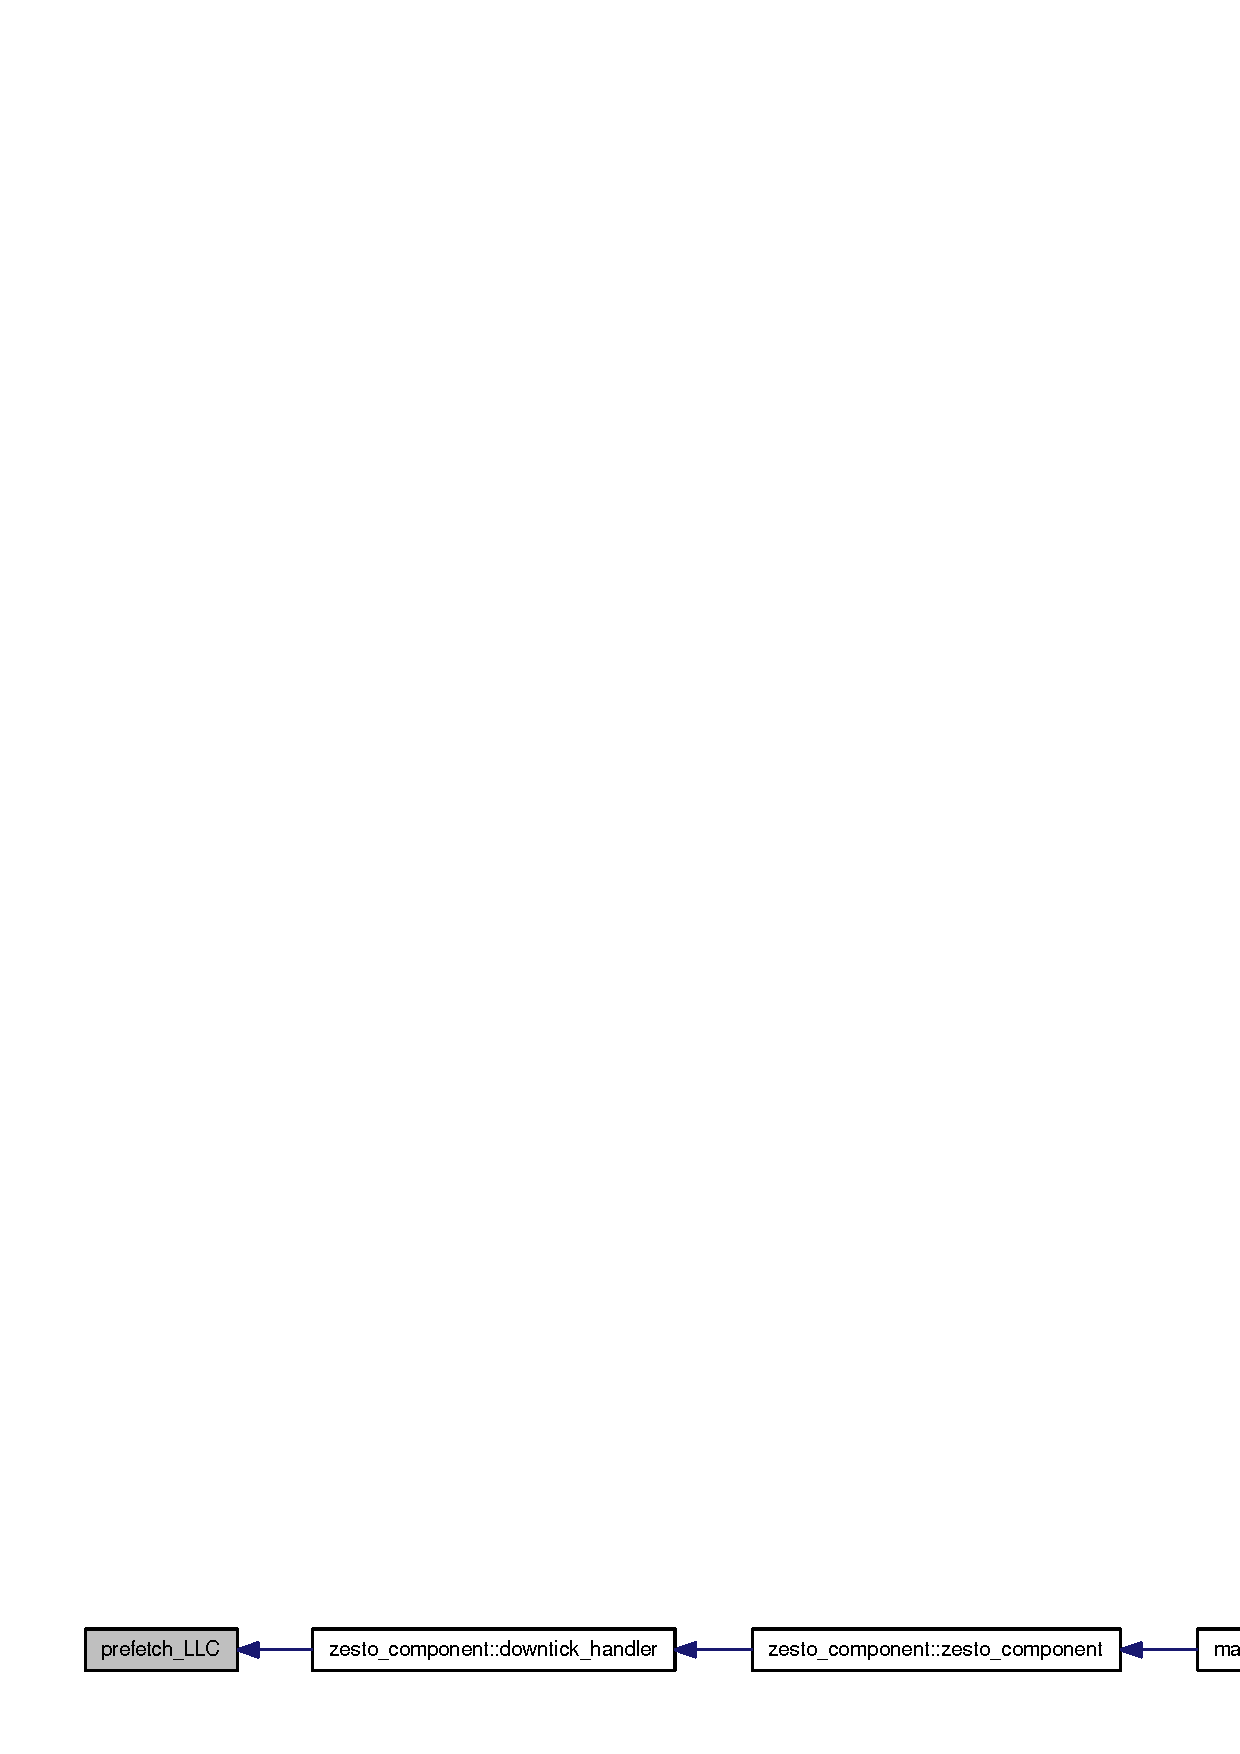
\includegraphics[width=308pt]{zesto-llc_8cpp_8ed5f90d7b07bddefbf6736b13da8eb2_icgraph}
\end{center}
\end{figure}
\index{zesto-llc.cpp@{zesto-llc.cpp}!step\_\-LLC\_\-PF\_\-controller@{step\_\-LLC\_\-PF\_\-controller}}
\index{step\_\-LLC\_\-PF\_\-controller@{step\_\-LLC\_\-PF\_\-controller}!zesto-llc.cpp@{zesto-llc.cpp}}
\subsubsection[{step\_\-LLC\_\-PF\_\-controller}]{\setlength{\rightskip}{0pt plus 5cm}void step\_\-LLC\_\-PF\_\-controller (struct {\bf uncore\_\-t} $\ast$const  {\em uncore})}\label{zesto-llc_8cpp_65086cfd5f54ff7a76a41587c8f6a01e}




Definition at line 2174 of file zesto-llc.cpp.

References uncore\_\-t::LLC, and prefetch\_\-controller\_\-update\_\-llc().

Referenced by zesto\_\-component::downtick\_\-handler().

Here is the caller graph for this function:\nopagebreak
\begin{figure}[H]
\begin{center}
\leavevmode
\includegraphics[width=331pt]{zesto-llc_8cpp_65086cfd5f54ff7a76a41587c8f6a01e_icgraph}
\end{center}
\end{figure}
\index{zesto-llc.cpp@{zesto-llc.cpp}!uncore\_\-utilize@{uncore\_\-utilize}}
\index{uncore\_\-utilize@{uncore\_\-utilize}!zesto-llc.cpp@{zesto-llc.cpp}}
\subsubsection[{uncore\_\-utilize}]{\setlength{\rightskip}{0pt plus 5cm}void uncore\_\-utilize (struct {\bf cache\_\-t} $\ast$const  {\em cp})}\label{zesto-llc_8cpp_d129e662a0b491f13301bf6f96bdcb8b}




Definition at line 2186 of file zesto-llc.cpp.

References cache\_\-t::stat, and cache\_\-t::uncore\_\-utilization.\index{zesto-llc.cpp@{zesto-llc.cpp}!WBB\_\-available@{WBB\_\-available}}
\index{WBB\_\-available@{WBB\_\-available}!zesto-llc.cpp@{zesto-llc.cpp}}
\subsubsection[{WBB\_\-available}]{\setlength{\rightskip}{0pt plus 5cm}static int WBB\_\-available (const struct {\bf cache\_\-t} $\ast$const  {\em cp}, \/  const {\bf md\_\-paddr\_\-t} {\em paddr})\hspace{0.3cm}{\tt  [inline, static]}}\label{zesto-llc_8cpp_48f8188c331e3c2188868d0f1c577d5a}




Definition at line 1086 of file zesto-llc.cpp.

References GET\_\-MSHR\_\-BANK, cache\_\-t::WBB\_\-num, and cache\_\-t::WBB\_\-size.\index{zesto-llc.cpp@{zesto-llc.cpp}!WBB\_\-insert@{WBB\_\-insert}}
\index{WBB\_\-insert@{WBB\_\-insert}!zesto-llc.cpp@{zesto-llc.cpp}}
\subsubsection[{WBB\_\-insert}]{\setlength{\rightskip}{0pt plus 5cm}static void WBB\_\-insert (struct {\bf cache\_\-t} $\ast$const  {\em cp}, \/  struct {\bf cache\_\-line\_\-t} $\ast$const  {\em cache\_\-block})\hspace{0.3cm}{\tt  [static]}}\label{zesto-llc_8cpp_54a68443796a201ceb5456ce0fc69bc4}




Definition at line 1096 of file zesto-llc.cpp.

References cache\_\-t::addr\_\-shift, cache\_\-line\_\-t::c\_\-state, cache\_\-assert, CACHE\_\-STAT, cache\_\-t::check\_\-for\_\-WBB\_\-work, cache\_\-t::check\_\-for\_\-work, cache\_\-line\_\-t::core, cache\_\-line\_\-t::dirty, GET\_\-MSHR\_\-BANK, mod2m(), modinc(), cache\_\-t::stat, cache\_\-line\_\-t::tag, cache\_\-line\_\-t::valid, cache\_\-line\_\-t::victim, cache\_\-t::WBB, cache\_\-t::WBB\_\-combines, cache\_\-t::WBB\_\-head, cache\_\-t::WBB\_\-insertions, cache\_\-t::WBB\_\-num, cache\_\-t::WBB\_\-size, cache\_\-t::WBB\_\-tail, and cache\_\-t::write\_\-combining.\index{zesto-llc.cpp@{zesto-llc.cpp}!WBB\_\-victim\_\-insert@{WBB\_\-victim\_\-insert}}
\index{WBB\_\-victim\_\-insert@{WBB\_\-victim\_\-insert}!zesto-llc.cpp@{zesto-llc.cpp}}
\subsubsection[{WBB\_\-victim\_\-insert}]{\setlength{\rightskip}{0pt plus 5cm}static void WBB\_\-victim\_\-insert (struct {\bf cache\_\-t} $\ast$const  {\em cp}, \/  struct {\bf cache\_\-line\_\-t} $\ast$const  {\em cache\_\-block})\hspace{0.3cm}{\tt  [static]}}\label{zesto-llc_8cpp_4a2ea45f307de25eaffcd48354e67a18}




Definition at line 1140 of file zesto-llc.cpp.

References cache\_\-t::addr\_\-shift, cache\_\-assert, CACHE\_\-STAT, cache\_\-line\_\-t::core, cache\_\-line\_\-t::dirty, GET\_\-MSHR\_\-BANK, mod2m(), cache\_\-t::stat, cache\_\-line\_\-t::tag, cache\_\-line\_\-t::valid, cache\_\-line\_\-t::victim, cache\_\-t::WBB, cache\_\-t::WBB\_\-head, cache\_\-t::WBB\_\-num, cache\_\-t::WBB\_\-size, and cache\_\-t::WBB\_\-victim\_\-insertions.